\documentclass{article}
\usepackage[margin=0.0cm,  left=0.0cm, paperwidth=18cm, paperheight=14cm]{geometry}
\usepackage{tikz}
\usetikzlibrary{shapes}
\usetikzlibrary{calc,backgrounds}
\usetikzlibrary{automata}
\usetikzlibrary{arrows,positioning,calc,matrix} 
\usetikzlibrary{decorations.pathreplacing,shapes.multipart}

\tikzstyle{Dstate}=[shape=circle,draw=black!50,fill=black!10]
\tikzstyle{Istate}=[shape=diamond,draw=black!50,fill=black!10]
\tikzstyle{Mstate}=[shape=rectangle,draw=black!50,fill=black!10]

\tikzstyle{empty}=[shape=circle]

\tikzstyle{lightedge}=[->,dotted,thick]
\tikzstyle{mainstate}=[state,thick]
\tikzstyle{mainedge}=[->,thick]

%\renewcommand{\chaptername}{}
%\renewcommand{\thechapter}{}

\definecolor{black}{RGB}{0,0,0}
\definecolor{darkgrey}{RGB}{64,64,64}
\definecolor{grey}{RGB}{127,127,127}
\definecolor{lightgrey}{RGB}{230,230,230}

% scheme 1 
\definecolor{winered}{RGB}{158,16,0}
\definecolor{lightred}{RGB}{199,53,42}
\definecolor{brown}{RGB}{158,95,0}
\definecolor{orange}{RGB}{235,141,0}

%scheme2

\definecolor{darkblue}{RGB}{19,48,182}

\definecolor{blue}{RGB}{36,89,158}
\definecolor{browngreen}{RGB}{82,75,19}
\definecolor{lightbrown}{RGB}{158,126,36}

%scheme3

\definecolor{green}{RGB}{52,132,23}


\definecolor{lightgreen}{RGB}{82,209,36}
\definecolor{lightbrowngreen}{RGB}{125,133,23}
\definecolor{yellowgreen}{RGB}{198,209,36}

%scheme4


\definecolor{paper}{RGB}{240,238,183}
\definecolor{organicgrey}{RGB}{163,162,124}


\definecolor{metal}{RGB}{75,81,82}
\begin{document}
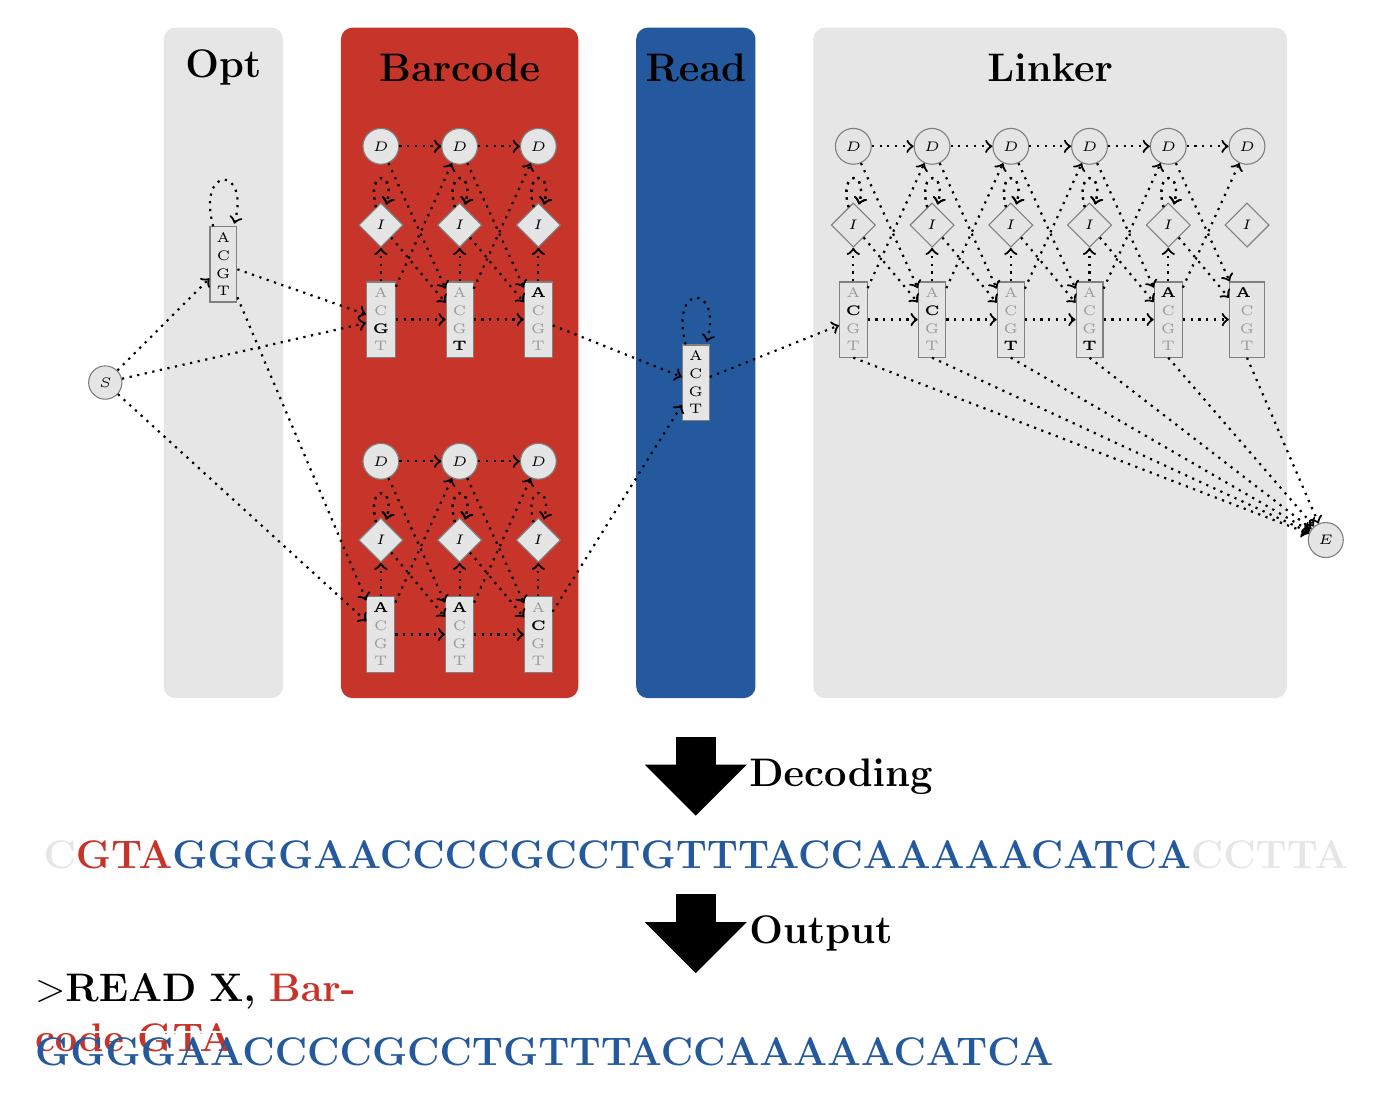
\begin{tikzpicture}[]
 \tiny

\draw[rounded corners=4pt,draw=lightgrey, fill=lightgrey] (-0.75,4.5)	rectangle (0.75,-4);

\draw[rounded corners=4pt,draw=lightred, fill=lightred] (1.5,4.5)	rectangle (4.5,-4);
 

\draw[rounded corners=4pt,draw=blue, fill=blue] (5.25,4.5)	rectangle (6.75,-4);
  
\draw[rounded corners=4pt,draw=lightgrey, fill=lightgrey] (7.5,4.5)	rectangle (13.5,-4);

 \node  at (0,4)  [font=\Large,style={align=center}] () {{\bf Opt}};
 
 \node  at (3,4)  [font=\Large,style={align=center}] () {{\bf Barcode}};
 
%  \node  at (3,2+1.75)  [font=\Large,style={align=center}] () {{\bf 1}};
  
 %   \node  at (3,-2+ 1.75)  [font=\Large,style={align=center}] () {{\bf 2}};
  \node  at (6,4)  [font=\Large,style={align=center}] () {{\bf Read}};
  
    \node  at (10.5,4)  [font=\Large,style={align=center}] () {{\bf Linker}};
    
\draw[
        -triangle 90,
        line width=2mm,
        postaction={draw, line width=0.5cm, shorten >=0.5cm, -}
    ] (6,-4.5) -- node[right=0.5,font =\Large] {{\bf Decoding}} (6,-5.5) ;
    
  \node[draw=white, thick,font=\Large] at (6,-6)  {\bf {\color{lightgrey}C}{\color{lightred}GTA}{\color{blue}GGGGAACCCCGCCTGTTTACCAAAAACATCA}{\color{lightgrey}CCTTA}} ;
  
  \draw[
        -triangle 90,
        line width=2mm,
        postaction={draw, line width=0.5cm, shorten >=0.5cm, -}
    ] (6,-6.5) -- node[right=0.5,font =\Large] {{\bf Output}} (6,-7.5) ;
  
  \node[style={align=left},text width=20em,draw=white, thick,font=\Large] at (0,-8)  {\bf  $>$READ X, {\color{lightred}Barcode GTA}  } ;
   \node[style={align=left},text width=20em,draw=white, thick,font=\Large] at (0,-8.5)  {\bf   {\color{blue}GGGGAACCCCGCCTGTTTACCAAAAACATCA}} ;
  
  
\begin{scope}[shift={(-1.5,0)}];
\node[Dstate] (START) at (0,0){$S$};
\end{scope}

\begin{scope}[shift={(0,1.5)}];
\node[Mstate] (O1) at (0,0){\shortstack{ A\\  C\\  G\\ T} };
\end{scope}

\begin{scope}[shift={(2,2)}];
\node[Dstate] (d1) at (0,1){$D$};
\node[Istate] (i1) at (0,0){$I$};
\node[Mstate] (m1) at (0,-1.2){\shortstack{ {\color{black!40}A}\\   {\color{black!40}C}\\  {\bf G}\\   {\color{black!40}T}} };



\node[Dstate] (d2) at (1,1){$D$};
\node[Istate] (i2) at (1,0){$I$};
\node[Mstate] (m2) at (1,-1.2){\shortstack{ {\color{black!40}A}\\   {\color{black!40}C}\\   {\color{black!40}G}\\   {\bf T}} };


\node[Dstate] (d3) at (2,1){$D$};
\node[Istate] (i3) at (2,-0){$I$};
\node[Mstate] (m3) at (2,-1.2){\shortstack{ {\bf A}\\   {\color{black!40}C}\\   {\color{black!40}G}\\   {\color{black!40}T}} };
\end{scope}


\begin{scope}[shift={(2,-2)}];

\node[Dstate] (d4) at (0,1){$D$};
\node[Istate] (i4) at (0,0){$I$};
\node[Mstate] (m4) at (0,-1.2){\shortstack{ {\bf A}\\   {\color{black!40}C}\\   {\color{black!40}G}\\   {\color{black!40}T}} };



\node[Dstate] (d5) at (1,1){$D$};
\node[Istate] (i5) at (1,0){$I$};
\node[Mstate] (m5) at (1,-1.2){\shortstack{ {\bf A}\\   {\color{black!40}C}\\   {\color{black!40}G}\\   {\color{black!40}T}} };


\node[Dstate] (d6) at (2,1){$D$};
\node[Istate] (i6) at (2,-0){$I$};
\node[Mstate] (m6) at (2,-1.2){\shortstack{ {\color{black!40}A}\\   {\bf C}\\   {\color{black!40}G}\\   {\color{black!40}T}} };
\end{scope}



\begin{scope}[shift={(6,0)}];



\node[Mstate] (R1) at (0,0){\shortstack{ A\\  C \\ G \\   T} };
\end{scope}



\begin{scope}[shift={(8,2)}];

%CCTTAAGG
\node[Dstate] (dl1) at (0,1){$D$};
\node[Istate] (il1) at (0,0){$I$};
\node[Mstate] (ml1) at (0,-1.2){\shortstack{ {\color{black!40}A}\\  {\bf C} \\   {\color{black!40}G}\\ {\color{black!40}T}} };



\node[Dstate] (dl2) at (1,1){$D$};
\node[Istate] (il2) at (1,0){$I$};
\node[Mstate] (ml2) at (1,-1.2){\shortstack{ {\color{black!40}A}\\   {\bf C}\\   {\color{black!40}G}\\   {\color{black!40}T}} };


\node[Dstate] (dl3) at (2,1){$D$};
\node[Istate] (il3) at (2,-0){$I$};
\node[Mstate] (ml3) at (2,-1.2){\shortstack{ {\color{black!40}A}\\   {\color{black!40}C}\\   {\color{black!40}G}\\   {\bf T}} };

\node[Dstate] (dl4) at (3,1){$D$};
\node[Istate] (il4) at (3,0){$I$};
\node[Mstate] (ml4) at (3,-1.2){\shortstack{ {\color{black!40}A}\\   {\color{black!40}C}\\   {\color{black!40}G}\\   {\bf T}} };

\node[Dstate] (dl5) at (4,1){$D$};
\node[Istate] (il5) at (4,0){$I$};
\node[Mstate] (ml5) at (4,-1.2){\shortstack{ {\bf A}\\   {\color{black!40}C}\\   {\color{black!40}G}\\   {\color{black!40}T}} };
\node[Dstate] (dl6) at (5,1){$D$};
\node[Istate] (il6) at (5,-0){$I$};
\node[Mstate] (ml6) at (5,-1.2){\shortstack{ {\bf A } \\   {\color{black!40}C}\\   {\color{black!40}G}\\   {\color{black!40}T}} };
\end{scope}

\begin{scope}[shift={(14,-2)}];
\node[Dstate] (END) at (0,0){$E$};
\end{scope}

 \path 
 
(START) edge [lightedge] (O1)

(START) edge [lightedge] (m1)

(START) edge [lightedge] (m4)
 
(O1) edge [lightedge, loop above] ()
(R1) edge [lightedge, loop above] ()
    
(O1)edge [lightedge] (m1)
(O1)edge [lightedge] (m4)
(R1)edge [lightedge] (ml1)

(ml1.south)edge [lightedge] (END)
(ml2.south)edge [lightedge] (END)
(ml3.south)edge [lightedge] (END)
(ml4.south)edge [lightedge] (END)
(ml5.south)edge [lightedge] (END)
(ml6.south)edge [lightedge] (END)


(m3)edge [lightedge] (R1)
(m6)edge [lightedge] (R1)

(m1) edge [lightedge] (m2) 
(m1) edge [lightedge] (d2) 
(m1) edge [lightedge] (i1)
   
(i1) edge [lightedge,loop above] ()
(i1) edge  [lightedge] (m2)
(i1) edge [lightedge, loop above] ()
(d1) edge  [lightedge,->] (d2)
(d1) edge  [lightedge,->] (m2)

(m2) edge [lightedge] (m3) 
(m2) edge [lightedge] (d3) 
(m2) edge [lightedge] (i2)
   
(i2) edge [lightedge,loop above] ()
(i2) edge  [lightedge] (m3)
(i2) edge [lightedge, loop above] ()
(d2) edge  [lightedge,->] (d3)
(d2) edge  [lightedge,->] (m3)


(m3) edge [lightedge] (i3)
   
(i3) edge [lightedge,loop above] ()

(i3) edge [lightedge, loop above] ()


(m4) edge [lightedge] (m5) 
(m4) edge [lightedge] (d5) 
(m4) edge [lightedge] (i4)
   
(i4) edge [lightedge,loop above] ()
(i4) edge  [lightedge] (m5)
(i4) edge [lightedge, loop above] ()
(d4) edge  [lightedge,->] (d5)
(d4) edge  [lightedge,->] (m5)

(m5) edge [lightedge] (m6) 
(m5) edge [lightedge] (d6) 
(m5) edge [lightedge] (i5)
   
(i5) edge [lightedge,loop above] ()
(i5) edge  [lightedge] (m6)
(i5) edge [lightedge, loop above] ()
(d5) edge  [lightedge,->] (d6)
(d5) edge  [lightedge,->] (m6)


(m6) edge [lightedge] (i6)
   
(i6) edge [lightedge,loop above] ()


 
(ml1) edge [lightedge] (ml2) 
(ml1) edge [lightedge] (dl2) 
(ml1) edge [lightedge] (il1)
   
(il1) edge [lightedge,loop above] ()
(il1) edge  [lightedge] (ml2)
(il1) edge [lightedge, loop above] ()
(dl1) edge  [lightedge,->] (dl2)
(dl1) edge  [lightedge,->] (ml2)

(ml2) edge [lightedge] (ml3) 
(ml2) edge [lightedge] (dl3) 
(ml2) edge [lightedge] (il2)
   
(il2) edge [lightedge,loop above] ()
(il2) edge  [lightedge] (ml3)
(il2) edge [lightedge, loop above] ()
(dl2) edge  [lightedge,->] (dl3)
(dl2) edge  [lightedge,->] (ml3)


(ml3) edge [lightedge] (ml4) 
(ml3) edge [lightedge] (dl4) 
(ml3) edge [lightedge] (il3)
   
(il3) edge [lightedge,loop above] ()
(il3) edge  [lightedge] (ml4)
(il3) edge [lightedge, loop above] ()
(dl3) edge  [lightedge,->] (dl4)
(dl3) edge  [lightedge,->] (ml4)


(ml4) edge [lightedge] (ml5) 
(ml4) edge [lightedge] (dl5) 
(ml4) edge [lightedge] (il4)
   
(il4) edge [lightedge,loop above] ()
(il4) edge  [lightedge] (ml5)
(il4) edge [lightedge, loop above] ()
(dl4) edge  [lightedge,->] (dl5)
(dl4) edge  [lightedge,->] (ml5)



(ml5) edge [lightedge] (ml6) 
(ml5) edge [lightedge] (dl6) 
(ml5) edge [lightedge] (il5)
   
(il5) edge [lightedge,loop above] ()
(il5) edge  [lightedge] (ml6)
(il5) edge [lightedge, loop above] ()
(dl5) edge  [lightedge,->] (dl6)
(dl5) edge  [lightedge,->] (ml6)
;

\end{tikzpicture}

\end{document}